
% ---------------------------------- Document Structure ----------------------------------
\documentclass[a4paper,11pt, notitlepage]{report}
\usepackage[top=1in, bottom=1.25in, left=1.125in, right=1.125in]{geometry}


% ---------------------------------- Packages  ----------------------------------
\usepackage{amsthm}
\usepackage{amssymb}
\usepackage{mathtools}			% Enhances amsmath
\usepackage{relsize}			% Greater range of text sizing options 
\usepackage{enumitem}			% Customize options for enumerate and itemize environments
\usepackage{bm}					% Bold symbols in math mode
\usepackage{bbm}				% mathbb for numbers
\usepackage{imakeidx}			% Index
\usepackage{float}				% Figure positioning
\usepackage{color, colortbl}	% Table colours
\usepackage{remreset} 			% Continue section counter on Chapter

\usepackage{changepage}			% Adjust margins mid document
\usepackage{caption}
\usepackage{listings}           % Inline code snippets
\usepackage{courier}

\renewcommand*\thesection{\arabic{section}}	
\setcounter{secnumdepth}{5}						% Allows chapter, section, subsection, subsubsection, pargraph, and subparagraph numbering

\definecolor{backcolour}{rgb}{0.95,0.95,0.92}
\lstdefinestyle{mystyle}{
    basicstyle=\ttfamily,
    backgroundcolor=\color{backcolour}
}
\lstset{style=mystyle}
\lstset{language=sql}

\usepackage[bookmarks]{hyperref}
\hypersetup{
    colorlinks=true,
    linkcolor=blue,
    filecolor=magenta,      
    urlcolor=black,
    citecolor=blue,
}

% ---------------------------------- Styles/Numbering for Theorems, etc. ----------------------------------
% Theorem, corollary, lemma, and remark formatting
%\theoremstyle{definition}
\newtheorem{theorem}{Theorem}[section]
\newtheorem{corollary}{Corollary}[theorem]
\newtheorem*{lemma}{Lemma}
\newtheorem*{remark}{Remark}
\renewcommand\qedsymbol{$\blacksquare$}
\theoremstyle{definition}
\newtheorem*{definition}{Definition}
\numberwithin{equation}{section}		% Number equations by section


\usepackage{titling}
\usepackage{blindtext}
\usepackage{lipsum}

% ---------------------------------- Document ----------------------------------
\author{
    Wong, Alexander\\
    \texttt{alex.wong@ualberta.ca}
}
\date{\today}
\title{CMPUT 663 Assignment 1: Overview of SOTorrent Data}


\begin{document}
\pagenumbering{arabic}

\maketitle
%\thispagestyle{empty}

\section{Introduction}
This assignment is an introduction to the 2019 Mining Software Repositories challenge data set \cite{DBLP:conf/msr/BaltesDT008}. StackOverflow Torrent (SOTorrent) provided \texttt{*.xml} and \texttt{*.csv} data is further imported into a \texttt{sqlite3} database for more effective querying and ER diagram generation \cite{wong_2019}. Original data was taken from the Stack Exchange Data Dump \cite{stackexchange}.

\section{Schema}

This section is meant to address \textbf{Question 1} of the assignment. Provided table schema definitions are \texttt{sqlite3} compatible. The data set is comprised of twenty tables. A full entity relationship diagram can be found in Figure \ref{fig:er-diagram}. StackOverflow schema column semantics is clarified by referencing Stack Exchange Data Dump \cite{se_schema_q}.

One thing that I expected to get from the schema was a separation of Questions and Answers into their own tables. In order to get this data, filtering on the Posts table is necessary.
\begin{lstlisting}
-- Select all Question posts
SELECT * FROM Posts WHERE PostTypeId=1;
SELECT * FROM Posts WHERE PostTypeId=(
    SELECT Id FROM PostType WHERE Type='Question'
);
-- Select all Answer posts
SELECT * FROM Posts WHERE PostTypeId=2;
SELECT * FROM Posts WHERE PostTypeId=(
    SELECT Id FROM PostType WHERE Type='Answer'
);
\end{lstlisting}

\begin{figure}[ht]
    \centering
    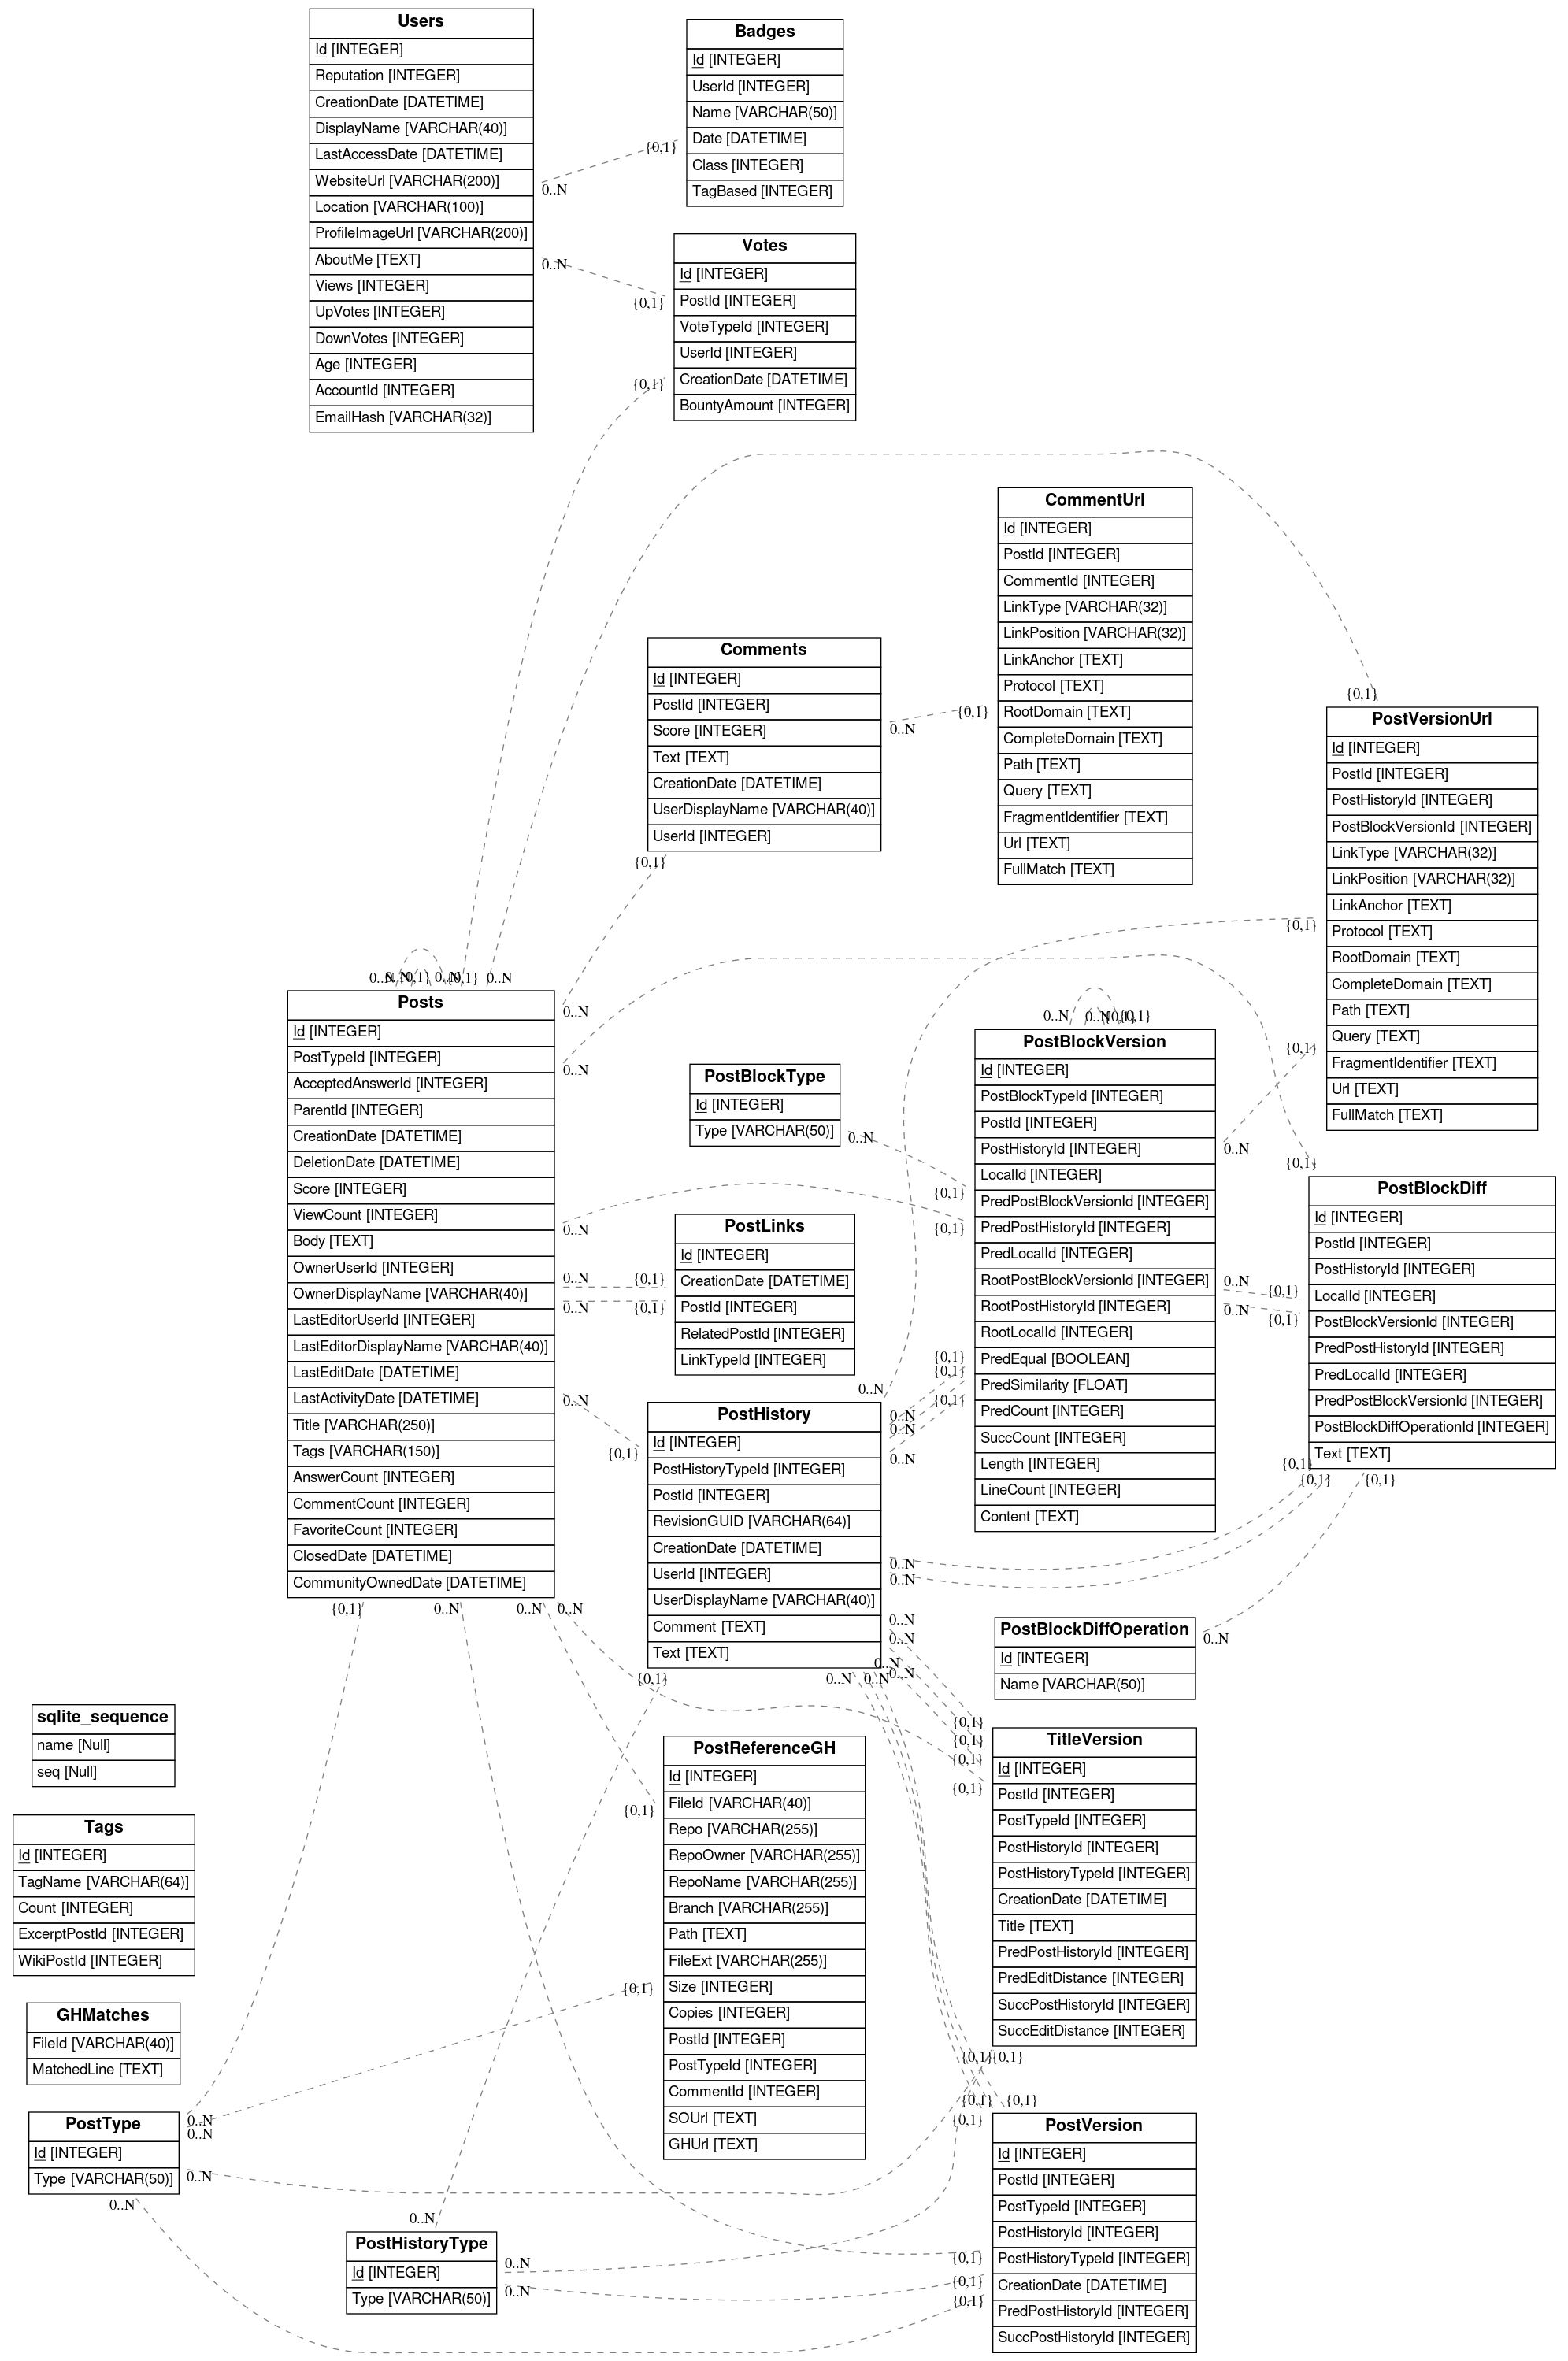
\includegraphics[width=6in]{figures/erd_from_sqlite.png}
    \caption{ER diagram of SOTorrent sqlite3 database using ERAlchemy \cite{eralchemy}.}
    \label{fig:er-diagram}
\end{figure}

\subsection{PostType}
\textbf{PostType} indicates the semantic type of a given Post.
\begin{lstlisting}
CREATE TABLE PostType (
    Id TINYINT NOT NULL,
    Type VARCHAR(50) NOT NULL,
    PRIMARY KEY(Id)
);
\end{lstlisting}
A single post may only have one post type. One post type entry may be used for multiple posts. All valid entries are $1$: \textit{Question}, $2$: \textit{Answer}, $3$: \textit{Wiki}, $4$: \textit{TagWikiExcerpt}, $5$: \textit{TagWiki}, $6$: \textit{ModeratorNomination}, $7$: \textit{WikiPlaceholder}, $8$: \textit{PrivilegeWiki}, $99$: \textit{Comment}. \textbf{PostType} data is provided directly from StackOverflow.

\subsection{PostHistoryType}
\textbf{PostHistoryType} indicate the semantic type of a modification to a given post.
\begin{lstlisting}
CREATE TABLE PostHistoryType (
    Id TINYINT NOT NULL,
    Type VARCHAR(50) NOT NULL,
    PRIMARY KEY(Id)
);
\end{lstlisting}
A single post history many only have one post history type. One post history type may be used for multiple post histories. All valid entries are $1$: \textit{Initial Title}, $2$: \textit{Initial Body}, $3$: \textit{Initial Tags}, $4$: \textit{Edit Title}, $5$: \textit{Edit Body}, $6$: \textit{Edit Tags}, $7$: \textit{Rollback Title}, $8$: \textit{Rollback Body}, $9$: \textit{Rollback Tags}, $10$: \textit{Post Closed}, $11$: \textit{Post Reopened}, $12$: \textit{Post Deleted}, $13$: \textit{Post Undeleted}, $14$: \textit{Post Locked}, $15$: \textit{Post Unlocked}, $16$: \textit{Community Owned}, $17$: \textit{Post Migrated}, $18$: \textit{Question Merged}, $19$: \textit{Question Protected}, $20$: \textit{Question Unprotected}, $22$: \textit{Question Unmerged}, $24$: \textit{Suggested Edit Applied}, $25$: \textit{Post Tweeted}, $31$: \textit{Discussion moved to chat}, $33$: \textit{Post Notice Added}, $34$: \textit{Post Notice Removed}, $35$: \textit{Post Migrated Away}, $36$: \textit{Post Migrated Here}, $37$: \textit{Post Merge Source}, $38$: \textit{Post Merge Destination}, or $50$: \textit{CommunityBump}. \textbf{PostHistoryType} data is provided directly from StackOverflow.

\subsection{Users}
\textbf{Users} hold the information for people using StackOverflow to ask and answer questions, as well as for posting comments and contributing votes.
\begin{lstlisting}
CREATE TABLE Users (
    Id INT NOT NULL,
    Reputation INT NOT NULL,
    CreationDate DATETIME,
    DisplayName VARCHAR(40),
    LastAccessDate DATETIME,
    WebsiteUrl VARCHAR(200),
    Location VARCHAR(100),
    ProfileImageUrl VARCHAR(200),
    AboutMe TEXT,
    Views INT DEFAULT 0,
    UpVotes INT,
    DownVotes INT,
    Age INT,
    AccountId INT,
    EmailHash VARCHAR(32),
    PRIMARY KEY (Id)
);
\end{lstlisting}
\textbf{Users} data is provided directly from StackOverflow.

\subsection{Badges}
\textbf{Badges} are given to users based on their activity on StackOverflow. The column \textit{Class} indicates the level of the provided badge, where $1$ is Gold, $2$ is Silver, and $3$ is Bronze. \textit{TagBased} badges are defined for contribution to non-community wiki answers and are awarded based on total accumulated score for the provided tag. For example, a user with a badge name \texttt{java} and class \texttt{1} is a Gold Java contributor. This user will have over 1000 cumulative score in at least 200 non-community wiki answers for the tag \texttt{java}.
\begin{lstlisting}
CREATE TABLE Badges (
    Id INT NOT NULL,
    UserId INT NOT NULL,
    Name VARCHAR(50),
    Date DATETIME,
    Class TINYINT,
    TagBased TINYINT(1),
    PRIMARY KEY (Id),
    FOREIGN KEY (UserId) REFERENCES Users(Id)
);
\end{lstlisting}
A single User may have zero to many badges. One row in Badges may only belong to a single user. \textbf{Badges} data is provided directly from StackOverflow.

\subsection{Posts}
\textbf{Posts} contain the primary data for StackOverflow. Refer to the \textbf{PostType} table for a complete list of all possible Posts.
\begin{lstlisting}
CREATE TABLE Posts (
    Id INT NOT NULL,
    PostTypeId TINYINT,
    AcceptedAnswerId INT,
    ParentId INT,
    CreationDate DATETIME,
    DeletionDate DATETIME,
    Score INT,
    ViewCount INT,
    Body TEXT,
    OwnerUserId INT,
    OwnerDisplayName VARCHAR(40),
    LastEditorUserId INT,
    LastEditorDisplayName VARCHAR(40),
    LastEditDate DATETIME,
    LastActivityDate DATETIME,
    Title VARCHAR(250),
    Tags VARCHAR(150),
    AnswerCount INT DEFAULT 0,
    CommentCount INT DEFAULT 0,
    FavoriteCount INT DEFAULT 0,
    ClosedDate DATETIME,
    CommunityOwnedDate DATETIME,
    PRIMARY KEY (Id),
    FOREIGN KEY (AcceptedAnswerId) REFERENCES Posts(Id),
    FOREIGN KEY (ParentId) REFERENCES Posts(Id),
    FOREIGN KEY (PostTypeId) REFERENCES PostType(Id)
);
\end{lstlisting}
A post may have a parent post. A post may also reference another post as an accepted answer. Relationships to Users and Tags are not enforced by a foreign key. Tags are stored as a single string of Tag Names encompassed by \texttt{<} and \texttt{>} symbols. \textbf{Posts} data is provided directly from StackOverflow.

\subsection{Comments}
\textbf{Comments} are discussion about a Post. Typically, discussion is about a provided question or a given answer that does not directly address the original question (like asking for clarification).
\begin{lstlisting}
CREATE TABLE Comments (
    Id INT NOT NULL,
    PostId INT NOT NULL,
    Score INT NOT NULL DEFAULT 0,
    Text TEXT,
    CreationDate DATETIME NOT NULL,
    UserDisplayName VARCHAR(40),
    UserId INT,
    PRIMARY KEY (Id),
    FOREIGN KEY (PostId) REFERENCES Posts(Id)
);
\end{lstlisting}
A comment must reference a single post. A post may have many comments. \textbf{Comments} data is provided directly from StackOverflow.

\subsection{PostHistory}
\textbf{PostHistory} are a record of changes to a Post after creation. Refer to the \textbf{PostHistoryType} table for a list of possible changes to a post.
\begin{lstlisting}
CREATE TABLE PostHistory (
    Id INT NOT NULL,
    PostHistoryTypeId TINYINT NOT NULL,
    PostId INT NOT NULL,
    RevisionGUID VARCHAR(64),
    CreationDate DATETIME,
    UserId INT,
    UserDisplayName VARCHAR(40),
    Comment TEXT,
    Text MEDIUMTEXT,
    PRIMARY KEY (Id),
    FOREIGN KEY (PostId) REFERENCES Posts(Id),
    FOREIGN KEY (PostHistoryTypeId) REFERENCES PostHistoryType(Id)
);
\end{lstlisting}
A post history entry must reference a single post and a single post history type. \textbf{PostHistory} data is provided directly from StackOverflow.

\subsection{PostLinks}
\textbf{PostLinks} are references from one StackOverflow post to another post. The field \textit{LinkTypeId} can have either value $1$ indicating a linked post, or $2$ indicating a duplicate post. PostLinks may only be assigned to Question type posts.
\begin{lstlisting}
CREATE TABLE PostLinks (
    Id INT NOT NULL,
    CreationDate DATETIME,
    PostId INT NOT NULL,
    RelatedPostId INT NOT NULL,
    LinkTypeId TINYINT,
    PRIMARY KEY (Id),
    FOREIGN KEY (PostId) REFERENCES Posts(Id),
    FOREIGN KEY (RelatedPostId) REFERENCES Posts(Id)
);
\end{lstlisting}
\textbf{PostLinks} data is provided directly from StackOverflow.

\subsection{Tags}
\textbf{Tags} are identifiers used to help distinguish a post. \textit{ExcerptPostId} is a reference to \textbf{Posts}, containing a short amount of text providing more information about the given tag. \textit{WikiPostId} is also a reference to \textbf{Posts}, but containing a more indepth wiki/knowledge base entry.
\begin{lstlisting}
CREATE TABLE Tags (
    Id INT NOT NULL,
    TagName VARCHAR(64),
    Count INT,
    ExcerptPostId INT,
    WikiPostId INT,
    PRIMARY KEY(Id)
);
\end{lstlisting}
\textbf{Tags} data is provided directly from StackOverflow.

\subsection{Votes}
\textbf{Votes} contain formation regarding a user's interaction with a post that is not encompassed by comments.
\begin{lstlisting}
CREATE TABLE Votes (
    Id INT NOT NULL,
    PostId INT NOT NULL,
    VoteTypeId TINYINT,
    UserId INT,
    CreationDate DATETIME,
    BountyAmount INT,
    PRIMARY KEY (Id),
    FOREIGN KEY (PostId) REFERENCES Posts(Id),
    FOREIGN KEY (UserId) REFERENCES Users(Id)
);
\end{lstlisting}
\textit{VoteTypeId} may be one of the following numbers: $1$ (AcceptedByOriginator), $2$ (UpMod (or upvote)), $3$ (DownMod (or downvote)), $4$ (Offensive), $5$ (Favorite (populates \textit{UserId})), $6$ (Close (as of 2013-06-25 stored in table \textit{PostHistory})), $7$ (Reopen), $8$ (BountyStart (populates \textit{UserId} and \textit{BountyAmount})), $9$ (BountyClose (populates \textit{BountyAmount}), $10$ (Deletion), $11$ (Undeletion), $12$ (Spam), $15$ (ModeratorReview), and $16$ (ApproveEditSuggestion). \textbf{Votes} data is provided directly from StackOverflow.

\subsection{PostBlockType}
\textbf{PostBlockType} indicate the semantic type of a \textbf{PostBlock}.
\begin{lstlisting}
CREATE TABLE PostBlockType (
    Id TINYINT NOT NULL,
    Type VARCHAR(50) NOT NULL,
    PRIMARY KEY(Id)
);
\end{lstlisting}
The two possible values are $1$: \texttt{TextBlock} or $2$: \texttt{CodeBlock}. \textbf{PostBlockType} data is generated from StackOverflow by the SOTorrent researchers.

\subsection{PostBlockDiffOperation}
\textbf{PostBlockDiffOperation} indicates the semantic type of a \textbf{PostBlockDiff}.
\begin{lstlisting}
CREATE TABLE PostBlockDiffOperation (
    Id TINYINT NOT NULL,
    Name VARCHAR(50) NOT NULL,
    PRIMARY KEY(Id)
);
\end{lstlisting}
The three possible values are $-1$: \texttt{DELETE}, $0$: \texttt{EQUAL}, or $3$: \texttt{INSERT}. \textbf{PostBlockDiffOperation} data is generated from StackOverflow by the SOTorrent researchers.

\subsection{PostVersion}
\textbf{PostVersion} shows the version history on the level of whole StackOverflow posts, or between two \textbf{PostHistory} entries.
\begin{lstlisting}
CREATE TABLE PostVersion (
    Id INTEGER PRIMARY KEY AUTOINCREMENT,
    PostId INT NOT NULL,
    PostTypeId TINYINT NOT NULL,
    PostHistoryId INT NOT NULL,
    PostHistoryTypeId TINYINT NOT NULL,
    CreationDate DATETIME NOT NULL,
    PredPostHistoryId INT DEFAULT NULL,
    SuccPostHistoryId INT DEFAULT NULL,
    UNIQUE(PostHistoryId, PredPostHistoryId, SuccPostHistoryId),
    FOREIGN KEY(PostId) REFERENCES Posts(Id),
    FOREIGN KEY(PostHistoryId) REFERENCES PostHistory(Id),
    FOREIGN KEY(PostTypeId) REFERENCES PostType(Id),
    FOREIGN KEY(PostHistoryTypeId) REFERENCES PostHistoryType(Id),
    FOREIGN KEY(PredPostHistoryId) REFERENCES PostHistory(Id),
    FOREIGN KEY(SuccPostHistoryId) REFERENCES PostHistory(Id)
);
\end{lstlisting}
\textbf{PostVersion} data is generated from StackOverflow by the SOTorrent researchers;

\subsection{PostBlockVersion}
\textbf{PostBlockVersion} shows the version history on the level of \textbf{PostBlocks}.
\begin{lstlisting}
CREATE TABLE PostBlockVersion (
    Id INTEGER PRIMARY KEY AUTOINCREMENT,
    PostBlockTypeId TINYINT NOT NULL,
    PostId INT NOT NULL,
    PostHistoryId INT NOT NULL,
    LocalId INT NOT NULL,
    PredPostBlockVersionId INT DEFAULT NULL,
    PredPostHistoryId INT DEFAULT NULL,
    PredLocalId INT DEFAULT NULL,
    RootPostBlockVersionId INT DEFAULT NULL,
    RootPostHistoryId INT DEFAULT NULL,
    RootLocalId INT DEFAULT NULL,
    PredEqual BOOLEAN DEFAULT NULL,
    PredSimilarity DOUBLE DEFAULT NULL,
    PredCount INT DEFAULT NULL,
    SuccCount INT DEFAULT NULL,
    Length INT NOT NULL,
    LineCount INT NOT NULL,
    Content TEXT NOT NULL,
    UNIQUE(PostHistoryId, PostBlockTypeId, LocalId),
    FOREIGN KEY(PostBlockTypeId) REFERENCES PostBlockType(Id),
    FOREIGN KEY(PostId) REFERENCES Posts(Id),
    FOREIGN KEY(PostHistoryId) REFERENCES PostHistory(Id),
    FOREIGN KEY(PredPostBlockVersionId)
        REFERENCES PostBlockVersion(Id),
    FOREIGN KEY(PredPostHistoryId) REFERENCES PostHistory(Id),
    FOREIGN KEY(RootPostBlockVersionId)
        REFERENCES PostBlockVersion(Id),
    FOREIGN KEY(RootPostHistoryId) REFERENCES PostHistory(Id)
);
\end{lstlisting}
\textbf{PostBlockVersion} data is generated from StackOverflow by the SOTorrent researchers;

\subsection{PostBlockDiff}
\textbf{PostBlockDiff} show the line based differences between two \textbf{PostBlock} entries.
\begin{lstlisting}
CREATE TABLE PostBlockDiff (
    Id INTEGER PRIMARY KEY AUTOINCREMENT,
    PostId INT NOT NULL,
    PostHistoryId INT NOT NULL,
    LocalId INT NOT NULL,
    PostBlockVersionId INT NOT NULL,
    PredPostHistoryId INT NOT NULL,
    PredLocalId INT NOT NULL,
    PredPostBlockVersionId INT NOT NULL,
    PostBlockDiffOperationId TINYINT NOT NULL,
    Text TEXT NOT NULL,
    FOREIGN KEY(PostId) REFERENCES Posts(Id),
    FOREIGN KEY(PostHistoryId) REFERENCES PostHistory(Id),
    FOREIGN KEY(PredPostHistoryId) REFERENCES PostHistory(Id),
    FOREIGN KEY(PostBlockDiffOperationId)
        REFERENCES PostBlockDiffOperation(Id),
    FOREIGN KEY(PostBlockVersionId)
        REFERENCES PostBlockVersion(Id),
    FOREIGN KEY(PredPostBlockVersionId)
        REFERENCES PostBlockVersion(Id)
);
\end{lstlisting}
\textbf{PostBlockDiff} data is generated from StackOverflow by the SOTorrent researchers;

\subsection{PostVersionUrl}
\textbf{PostVersionUrl} are URL links extracted from the text block versions.
\begin{lstlisting}
CREATE TABLE PostVersionUrl (
    Id INTEGER PRIMARY KEY AUTOINCREMENT,
    PostId INT NOT NULL,
    PostHistoryId INT NOT NULL,
    PostBlockVersionId INT NOT NULL,
    LinkType VARCHAR(32) NOT NULL,
    LinkPosition VARCHAR(32) NOT NULL,
    LinkAnchor TEXT DEFAULT NULL,
    Protocol TEXT NOT NULL,
    RootDomain TEXT NOT NULL,
    CompleteDomain TEXT NOT NULL,
    Path TEXT DEFAULT NULL,
    Query TEXT DEFAULT NULL,
    FragmentIdentifier TEXT DEFAULT NULL,
    Url TEXT NOT NULL,
    FullMatch TEXT NOT NULL,
    FOREIGN KEY(PostId) REFERENCES Posts(Id),
    FOREIGN KEY(PostHistoryId) REFERENCES PostHistory(Id),
    FOREIGN KEY(PostBlockVersionId)
        REFERENCES PostBlockVersion(Id)
);
\end{lstlisting}
\textbf{PostVersionUrl} data is generated from StackOverflow by the SOTorrent researchers;

\subsection{CommentUrl}
\textbf{CommentUrl} are URL links extracted from the post comments.
\begin{lstlisting}
CREATE TABLE CommentUrl (
    Id INTEGER PRIMARY KEY AUTOINCREMENT,
    PostId INT NOT NULL,
    CommentId INT NOT NULL,
    LinkType VARCHAR(32) NOT NULL,
    LinkPosition VARCHAR(32) NOT NULL,
    LinkAnchor TEXT DEFAULT NULL,
    Protocol TEXT NOT NULL,
    RootDomain TEXT NOT NULL,
    CompleteDomain TEXT NOT NULL,
    Path TEXT DEFAULT NULL,
    Query TEXT DEFAULT NULL,
    FragmentIdentifier TEXT DEFAULT NULL,
    Url TEXT NOT NULL,
    FullMatch TEXT NOT NULL,
    FOREIGN KEY(CommentId) REFERENCES Comments(Id)
);
\end{lstlisting}
\textbf{CommentUrl} data is generated from StackOverflow by the SOTorrent researchers;

\subsection{PostReferenceGH}
\textbf{PostReferenceGH} contain URLs extracted from GitHub which point to StackOverflow questions, answers, or comments. The column \textit{Copies} indicate how often the given \textit{FileId} appears in this table.
\begin{lstlisting}
CREATE TABLE PostReferenceGH (
    Id INTEGER PRIMARY KEY AUTOINCREMENT,
    FileId VARCHAR(40) NOT NULL,
    Repo VARCHAR(255) NOT NULL,
    RepoOwner VARCHAR(255) NOT NULL,
    RepoName VARCHAR(255) NOT NULL,
    Branch VARCHAR(255) NOT NULL,
    Path TEXT NOT NULL,
    FileExt VARCHAR(255) NOT NULL,
    Size INT NOT NULL,
    Copies INT NOT NULL,
    PostId INT NOT NULL,
    PostTypeId TINYINT NOT NULL,
    CommentId INT DEFAULT NULL,
    SOUrl TEXT NOT NULL,
    GHUrl TEXT NOT NULL,
    FOREIGN KEY(PostId) REFERENCES Posts(Id),
    FOREIGN KEY(PostTypeId) REFERENCES PostType(Id)
);
\end{lstlisting}
\textbf{PostReferenceGH} data is generated from StackOverflow and GitHub by the SOTorrent researchers;

\subsection{TitleVersion}
\textbf{TitleVersion} show the version history of StackOverflow question titles.
\begin{lstlisting}
REATE TABLE TitleVersion (
    Id INTEGER PRIMARY KEY AUTOINCREMENT,
    PostId INT NOT NULL,
    PostTypeId TINYINT NOT NULL,
    PostHistoryId INT NOT NULL,
    PostHistoryTypeId TINYINT NOT NULL,
    CreationDate DATETIME NOT NULL,
    Title TEXT NOT NULL,
    PredPostHistoryId INT DEFAULT NULL,
    PredEditDistance INT DEFAULT NULL,
    SuccPostHistoryId INT DEFAULT NULL,
    SuccEditDistance INT DEFAULT NULL,
    UNIQUE(PostHistoryId, PredPostHistoryId, SuccPostHistoryId),
    FOREIGN KEY(PostId) REFERENCES Posts(Id),
    FOREIGN KEY(PostTypeId) REFERENCES PostType(Id),
    FOREIGN KEY(PostHistoryId) REFERENCES PostHistory(Id),
    FOREIGN KEY(PostHistoryTypeId) REFERENCES PostHistoryType(Id),
    FOREIGN KEY(PredPostHistoryId) REFERENCES PostHistory(Id),
    FOREIGN KEY(SuccPostHistoryId) REFERENCES PostHistory(Id)
);
\end{lstlisting}
\textbf{TitleVersion} data is generated from StackOverflow by the SOTorrent researchers.

\subsection{GHMatches}
\textbf{GHMatches} contain the matched lines of source code from GitHub, used to create the \textbf{PostReferenceGH} table.
\begin{lstlisting}
CREATE TABLE GHMatches (
    FileId VARCHAR(40) NOT NULL,
    MatchedLine LONGTEXT NOT NULL
);
\end{lstlisting}
\textbf{GHMatches} is generated from GitHub by the SOTorrent researchers.

\section{Size Metrics and Traceability}

The remainder of the document shows the various Size and Traceability metrics as requested by the assignment.

\begin{itemize}
    \item Total counts of parsed entities can be found in Table \ref{table-counts}. Counts of posts by \texttt{PostTypes} can be found in Table \ref{post-type-counts}.
    \item Statistics of authored posts for questions, answers, and comments can be found in Figure \ref{fig:author-to-num-entiies} and Table \ref{table:author-to-num-entities}.
    \item Statistics of post blocks, including number of blocks and lines can be found in Figures \ref{fig:post-block-version-length-boxplot}, \ref{fig:post-block-version-linecount-boxplot} and Table \ref{tab:post-block-version-stats}.
    \item Count of foreign URLs parsed from comments and posts can be found in Table \ref{tab:foreign-urls}.
    \item Posts and corresponding number of answers can be found in Figure \ref{fig:questions-to-num-answers} and Table \ref{table:questions-to-num-answers}.
    \item Count of Python snippets is approximated in Table \ref{tab:python-snippets-summary}. Code analysis of PostBlockVersion content is \textbf{not} performed. From Posts, I selected all PostIds of questions that had the tag \texttt{python}. I then selected all PostIds for answers that answered the previously selected questions. Combining these two sets of PostIds, I performed summary statistics on the PostBlockVersion where the PostId was contained in this set. This provides an upper bound for possible number of Python code snippets, which I will better calculate in my MSR challenge paper.
    \item Rarest badges can be found in Table \ref{tab:rarest-badges}. Popular badges over time can be found in Figure \ref{fig:popular-badges-over-time}.
    \item Questions and answers over time can be found in Figure \ref{fig:q-and-a-over-time}.
    \item Popular tags over time can be found in Figure \ref{fig:popular-tags-over-time}.
\end{itemize}

\begin{table}[ht]
\centering
\begin{tabular}{rl}
\hline
\textbf{Table Name}     & \textbf{Number of Rows}   \\ \hline
Badges                  & 29307838                  \\
CommentUrl              & 7313266                   \\
Comments                & 70206499                  \\
GHMatches               & 588012                    \\
PostBlockDiff           & 155753959                 \\
PostBlockDiffOperation  & 3                         \\
PostBlockType           & 2                         \\
PostBlockVersion        & 212260401                 \\
PostHistory             & 112411821                 \\
PostHistoryType         & 31                        \\
PostLinks               & 5497178                   \\
PostReferenceGH         & 6111157                   \\
PostType                & 9                         \\
PostVersion             & 67466517                  \\
PostVersionUrl          & 33580154                  \\
Posts                   & 42850538                  \\
Tags                    & 53806                     \\
TitleVersion            & 19419656                  \\
Users                   & 9737247                   \\
Votes                   & 161605822                 \\
\end{tabular}
\caption{Count of rows per table: \texttt{SELECT COUNT(*) FROM \{Table Name\};}}
\label{table-counts}
\end{table}

\begin{table}[ht]
\centering
\begin{tabular}{rl}
\hline
\textbf{Post Type}      & \textbf{Number of Posts}  \\ \hline
Question            & 16845942  \\
Answer              & 25908201  \\
Wiki                & 167       \\
TagWikiExcerpt      & 47955     \\
TagWiki             & 47955     \\
ModeratorNomination & 312       \\
WikiPlaceholder     & 4         \\
PrivilegeWiki       & 2         \\
\end{tabular}
\caption{Count of Posts by PostTypes: \texttt{SELECT COUNT(PostTypeId), PostTypeId from Posts GROUP BY PostTypeId;}}
\label{post-type-counts}
\end{table}

\begin{table}[ht]
\centering
\begin{tabular}{r|cc|cc|c}
\hline
& \multicolumn{2}{c}{\textbf{Owned}} & \multicolumn{2}{c}{\textbf{Edited}} & \textbf{Written} \\
\textbf{Statistic} & \textbf{Questions} & \textbf{Answers} & \textbf{Questions} & \textbf{Answers} & \textbf{Comments} \\ \hline
Minimum Count       & 1     & 1     & 1     & 1     & 1     \\
1st Quartile        & 1     & 1     & 1     & 1     & 2     \\
Median              & 2     & 2     & 1     & 2     & 4     \\
Mean                & 5.152 & 12.61 & 6.64  & 10.35 & 26.09 \\
3rd Quartile        & 4     & 5     & 3     & 5     & 12    \\
Maximum Count       & 2391  & 50481 & 77720 & 26227 & 96314 \\ \hline
Number of Authors   & 3221661 & 2037004 & 1286402 & 661496 & 2658479 \\
\end{tabular}
\caption{User summary statistics for authoring Questions, Answers, and Comments. Only entities with valid User Ids (greater than 0) were considered.}
\label{table:author-to-num-entities}
\end{table}

\begin{figure}[ht]
    \centering
    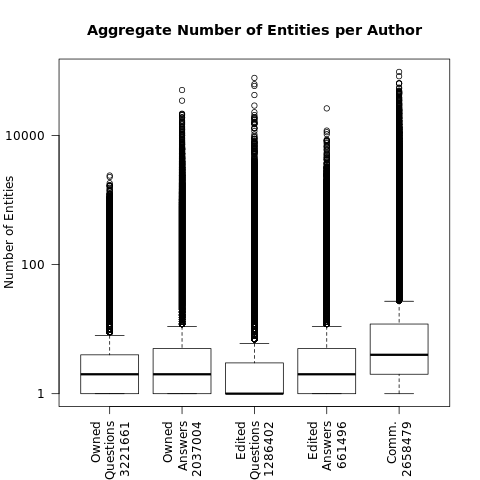
\includegraphics[width=6in]{figures/num_entities_per_author.png}
    \caption{Count of valid authors for Questions, Answers, and Comments. See Table \ref{table:author-to-num-entities}.}
    \label{fig:author-to-num-entiies}
\end{figure}

\begin{table}[]
    \centering
    \begin{tabular}{c|cc|cc}
    \hline
    & \multicolumn{2}{c}{\textbf{Text Block}} & \multicolumn{2}{c}{\textbf{Code Block}} \\
    \textbf{Statistic} & \textbf{Length} & \textbf{Line Count} & \textbf{Length} & \textbf{Line Count} \\ \hline
    Minimum         & 1     & 1     & 1     & 1     \\
    1st Quartile    & 61    & 1     & 85    & 2     \\
    Median          & 154   & 2     & 204   & 6     \\
    Mean            & 257.2 & 2.638 & 481.1 & 12.64 \\
    3rd Quartile    & 325   & 3     & 487   & 14    \\
    Maximum         & 29996 & 3837  & 29747 & 2576  \\ \hline
    Count Rows      & \multicolumn{2}{c}{129790412} & \multicolumn{2}{c}{82469989} \\
    \end{tabular}
    \caption{Summary statistics for PostBlockVersions by PostBlockType.}
    \label{tab:post-block-version-stats}
\end{table}

\begin{figure}[ht]
    \centering
    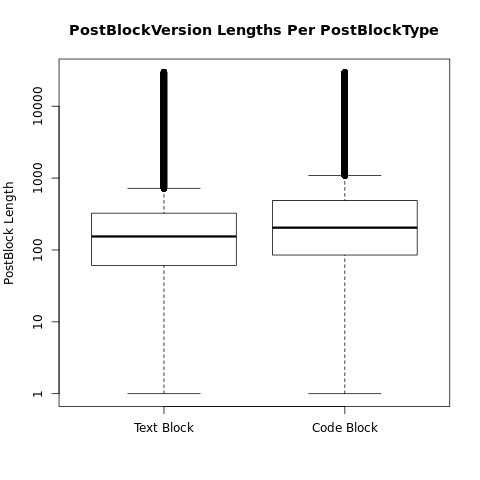
\includegraphics[width=6in]{figures/post_block_version_length_boxplot.png}
    \caption{Boxplot of the post block version lengths per type. See Table \ref{tab:post-block-version-stats}.}
    \label{fig:post-block-version-length-boxplot}
\end{figure}

\begin{figure}[ht]
    \centering
    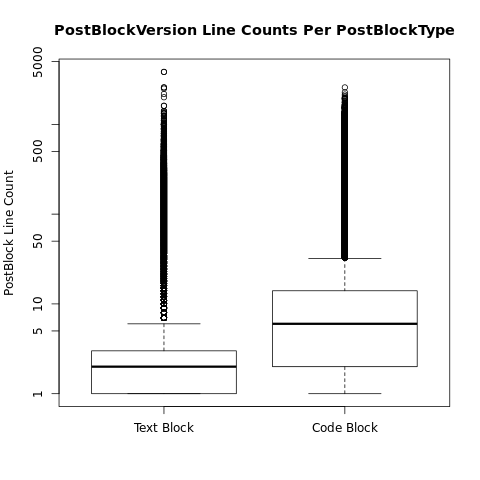
\includegraphics[width=6in]{figures/post_block_version_linecount_boxplot.png}
    \caption{Boxplot of the post block version line counts per type. See Table \ref{tab:post-block-version-stats}.}
    \label{fig:post-block-version-linecount-boxplot}
\end{figure}

\begin{table}[ht]
    \centering
    \begin{tabular}{cc|cc}
    \hline \multicolumn{2}{c}{\textbf{Comment}} & \multicolumn{2}{c}{\textbf{PostVersion}} \\
    \textbf{Root Domain} & \textbf{Count} & \textbf{Root Domain} & \textbf{Count} \\ \hline
    \texttt{stackoverflow.com} & 2428905 & \texttt{stackoverflow.com} & 5122628 \\
    \texttt{github.com} & 461133 & \texttt{imgur.com} & 4299090 \\
    \texttt{jsfiddle.net} & 325217 & \texttt{github.com} & 2278076 \\
    \texttt{microsoft.com} & 280454 & \texttt{microsoft.com} & 1639028\\
    \texttt{stackexchange.com} & 149757 & \texttt{jsfiddle.net} & 1362618 \\
    \texttt{google.com} & 149218 & \texttt{wikipedia.org} & 875390 \\
    \texttt{wikipedia.org} & 141293 & \texttt{google.com} & 848032 \\
    \texttt{php.net} & 124745 & \texttt{oracle.com} & 620087 \\
    \texttt{oracle.com} & 106253 & \texttt{php.net} & 485568 \\
    \texttt{mozilla.org} & 81330 & \texttt{python.org} & 425719 \\ 
    \multicolumn{2}{c}{\vdots} & \multicolumn{2}{c}{\vdots} \\ \hline
    Total Number Rows & 7313266 & Total Number Rows & 33580154 \\
    Count Foreign URLs & 4884361 & Count Foreign URLs & 28457526 \\
    \end{tabular}
    \caption{Top ten root domain counts of URLs for comments and posts. Count foreign URLs are obtained by subtracting the number of \texttt{stackoverflow.com} URLs from the total number of rows.}
    \label{tab:foreign-urls}
\end{table}

\begin{table}[ht]
\centering
\begin{tabular}{rc}
\hline
\textbf{Statistic} & \textbf{Number of Answers per Question} \\ \hline
Minimum Count   & 0 \\
1st Quartile    & 28.25 \\
Median          & 56.50 \\
Mean            & 72.33 \\
3rd Quartile    & 87.75 \\
Maximum Count   & 518   \\
\end{tabular}
\caption{Summary statistics of questions and their corresponding number of answers. There are 2261213 questions that remain unanswered.}
\label{table:questions-to-num-answers}
\end{table}

\begin{figure}[ht]
    \centering
    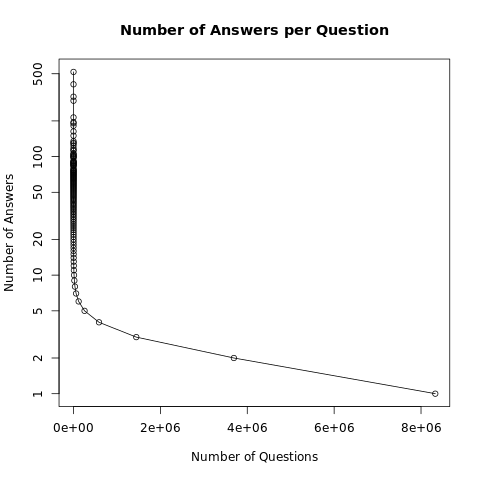
\includegraphics[width=6in]{figures/num_ans_per_question.png}
    \caption{Count of questions and their corresponding number of answers. There are 2261213 questions that remain unanswered.}
    \label{fig:questions-to-num-answers}
\end{figure}

\begin{table}[ht]
    \centering
    \begin{tabular}{r|cc}
    \hline
    \textbf{Statistic} & \textbf{Length} &\textbf{Line Count} \\ \hline
    Minimum         & 1     & 1     \\  
    1st Quartile    & 75    & 2     \\
    Median          & 172   & 5     \\
    Mean            & 378.5 & 9.751 \\
    3rd Quartile    & 394   & 11    \\
    Maximum         & 29613 & 2066  \\ \hline
    Upper Bound of Python Code Snippet Count & \multicolumn{2}{c}{6834349} \\
    \end{tabular}
    \caption{Summary statistics of PostBlockVersions where the related Post was tagged with \texttt{python}. Posts of type Question are tagged with \texttt{python}. Posts of type Answer are untagged, but are counted in the above table when the entity answers a Question that has been tagged with \texttt{python}.}
    \label{tab:python-snippets-summary}
\end{table}

\begin{table}[ht]
    \centering
    \begin{tabular}{c|cc}
    \hline
    \textbf{Badge Name} & \textbf{Class} & \textbf{Recipients} \\ \hline
    Sheriff & Gold & 39 \\
    Illuminator & Gold & 100 \\
    Legendary & Gold & 260 \\
    Documentation Beta & Silver & 293 \\
    Reversal & Gold & 298 \\
    Research Assistant & Silver & 299 \\
    Epic & Silver & 674 \\
    Synonymizer & Bronze & 945 \\
    Not a Robot & Silver & 1003 \\
    Generalist & Silver & 1019 \\
    \end{tabular}
    \caption{Top ten rarest non tag-based badges on Stack Overflow. Tag-based badges have many tags where only a single user has been awared the badge.}
    \label{tab:rarest-badges}
\end{table}

\begin{figure}[ht]
    \centering
    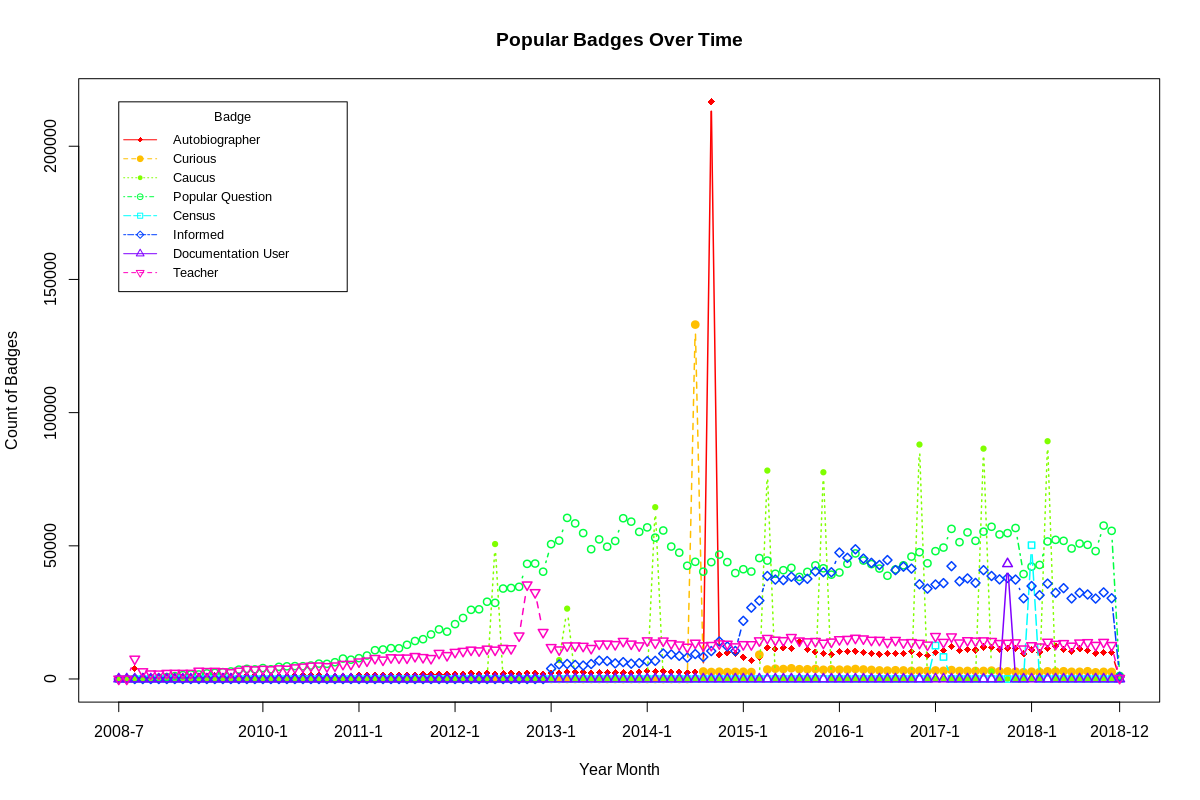
\includegraphics[angle=270,width=5.5in]{figures/popular_badges_over_time.png}
    \caption{Top eight popular badges over time. Each point represents a sum of the Bronze, Silver, and Gold classes for the badge name awarded in the given year/month.}
    \label{fig:popular-badges-over-time}
\end{figure}

\begin{figure}[ht]
    \centering
    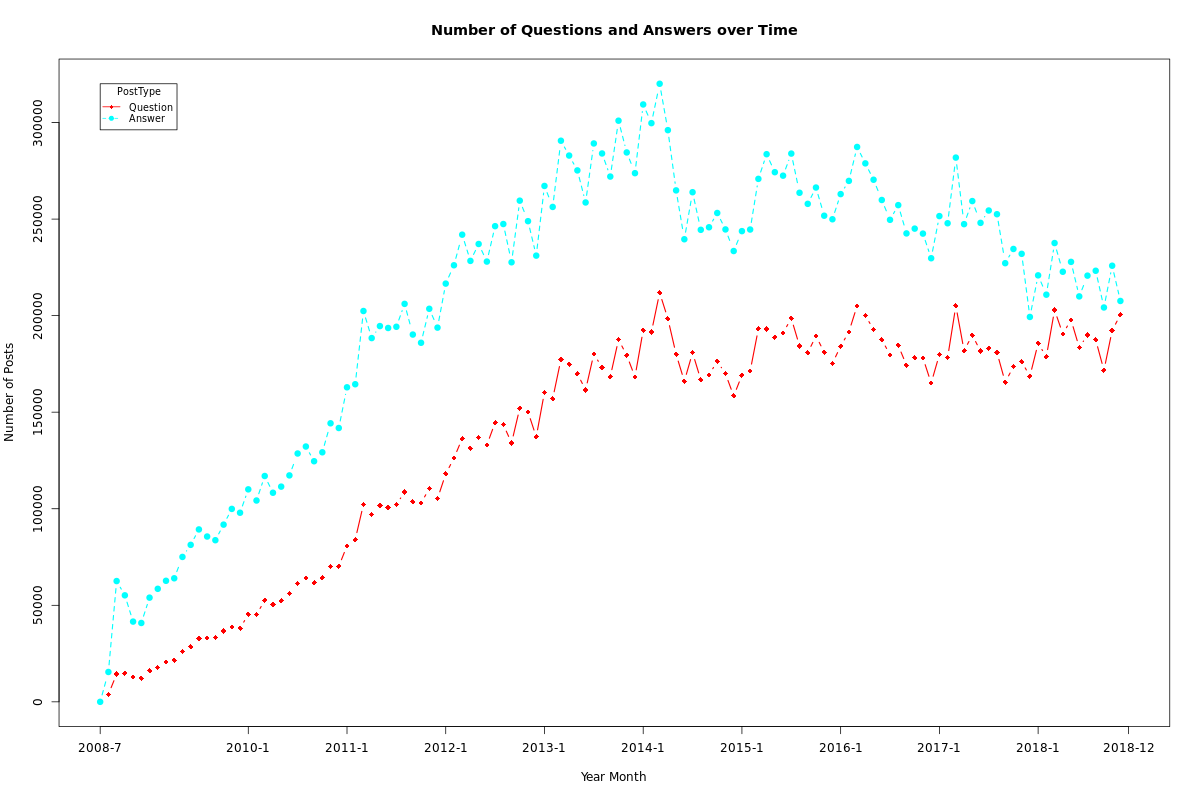
\includegraphics[angle=270,width=5.5in]{figures/num_q_and_a_over_time.png}
    \caption{Number of questions and answers over time. Each point represents a sum for the given year/month.}
    \label{fig:q-and-a-over-time}
\end{figure}

\begin{figure}[ht]
    \centering
    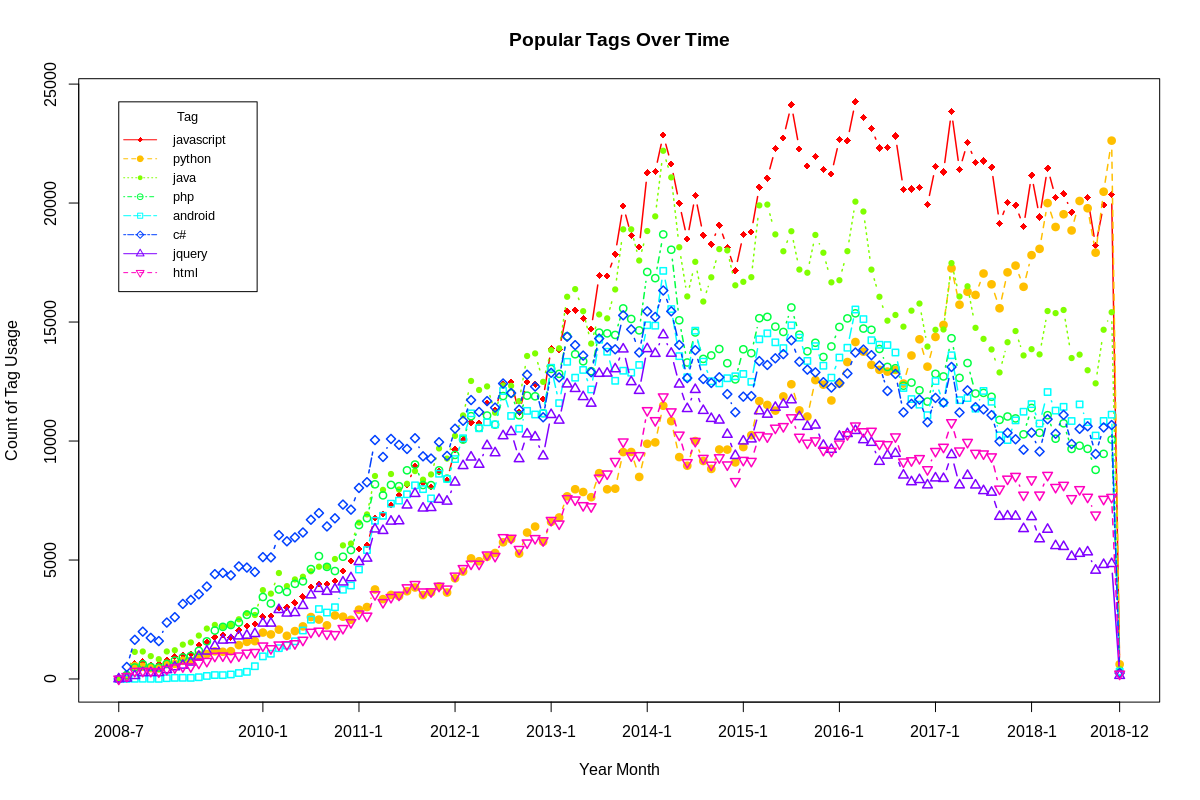
\includegraphics[angle=270,width=5.5in]{figures/popular_tags_over_time.png}
    \caption{Top eight popular tags over time. Each point represents a sum of the count of questions with the tag for the given year/month.}
    \label{fig:popular-tags-over-time}
\end{figure}


\bibliographystyle{ieeetr}
\bibliography{references} % Entries are in the "references.bib" file

\end{document}
